\subsection{Kombinatorische Aspekte}
\paragraph{Entsperrmuster}
(in Bezug auf Nummerierung auf Abb. 1 der Angabe) \\

In \ref{bild1} sind die Überlegungen der Möglichkeiten als grobe Skizze festgehalten. Als Startmöglichkeiten sind die Kombinationen 1-2, 1-4, 1-5, 1-6 und 1-8 möglich. 1-3, 1-7 und 1-9 sind nicht direkt möglich, da auf der geraden Linie zuerst über andere Knoten gelaufen wird, die zuerst markiert werden würden. Die Überlegungen für 1-2 und 1-6 können wegen der Symmetrie entlang der Diagonale für die Starts mit 1-4 bzw. 18 übernommen werden. Damit kommt man auf folgende Anzahl der Möglichkeiten:
\begin{equation}
\centering
\begin{aligned}
anzahl(1-2) \cdot 2 + anzahl(1-5) + anzahl(1-6) \cdot 2 = \\
(4+5+6+5+4+4) \cdot 2 + (6+5+6+6+5+6+4) + (5+5+6+4+5+5) \cdot 2 = 154
\end{aligned}
\end{equation}

\begin{figure}
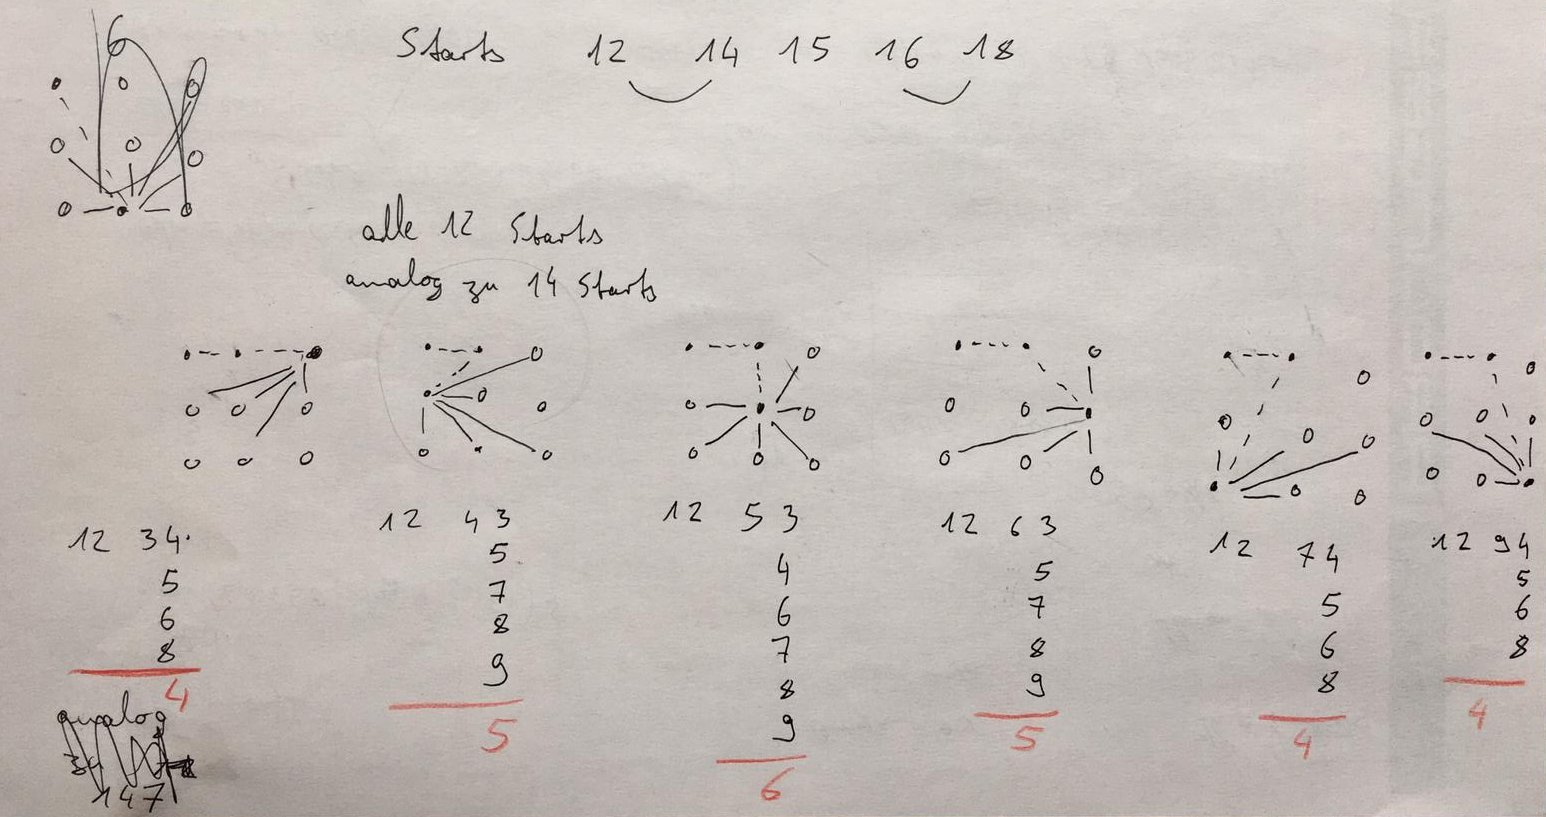
\includegraphics[width=7cm]{bilder/1.jpeg}
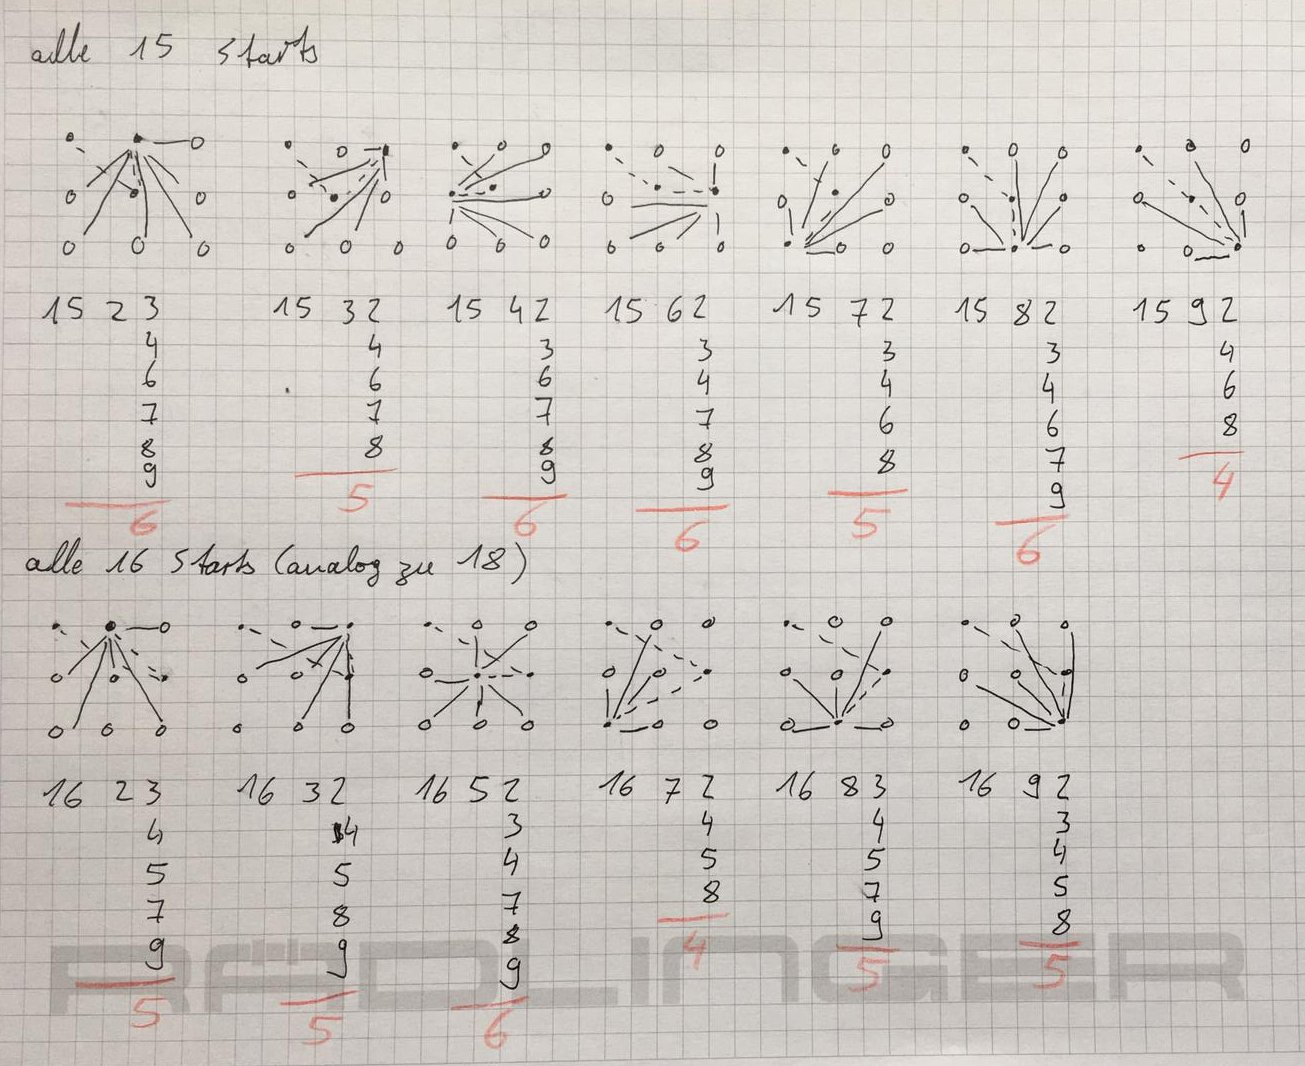
\includegraphics[width=7cm]{bilder/2.jpeg}
\centering
\caption{kombinatorisches Abzählen der Möglichkeiten}
\label{bild1}
\end{figure}

\paragraph{PINn}
4 Stellen, erste Ziffer ist 1 \\
Anzahl an Möglichkeiten:
\begin{equation}
1 \cdot 10 \cdot 10 \cdot 10 = 1000
\end{equation}

\subsection{Angriffsmöglichkeiten}

\begin{itemize}
\item klassischer over-the-shoulder Angriff durch Zuschauen -> direktes Ablesen
\item Finger hinterlässt Wischspur auf Bildschirm, wenn dann etwa nur entsperrt wird und nicht auf dem Bildschirm weitergewischt wird, kann der Angreifer den Weg des Musters nachvollziehen
\item indirektes Abschauen/Eingrenzen der Möglichkeiten durch Beobachtung der Haltung der Hand, Bewegung des Fingers etc -> allerdings nur begrenzt möglich, da sich das Handy meistens nach zu vielen Fehlversuchen sperrt
\end{itemize}

\subsection{Beispielstudie}
zwei Gruppen: Nutzer mit PINn bzw. Lock Pattern Abfrage beim Entsperren des Smartphones
Die Teilnehmer werden zu Studienbeginn einer Gruppe (PINn/Pattern) zugeordnet und legen demnach selbst entsprechend ihrer Gruppe einen PIN/Muster fest. Eine App zählt über die Ausführungsdauer der Studie die jeweilige Anzahl an Fehlversuchen bis zum erfolgreichen Entsperren mit (in Bezug auf Usability der Sicherheitsmaßnahme). \\
Am Ende der Studie werden die PINns und Muster der Teilnehmer rein stochastisch/kombinatorisch auf Sicherheit ausgewertet. Dazu wird bei einem "Zwischengespräch" wird unter nicht-Wissen der Teilnehmer ein over-the-shoulder-Angriff simuliert und auf Erfolg getestet. \\
Bei der Auswertung werden dann die verschiedenen Faktoren zusammengeführt und verglichen. Sprich, ist ein "rein mathematisch" sichereres Verfahren für solche "Alltagsangriffszenarien" auch wirklich effektiver? Wie verhält es sich mit Benutzbarkeit zwischen den beiden Verfahren, auch im Zusammenhang mit dem Grad an Sicherheit?

\paragraph{Sicherheitsziele und Angreifermodell}
\begin{itemize}
\item Sicherheitsziel: angemessener Grad an "Aufwand" für den Nutzer für Schutz gegen "alltägliche" Angriffe auf Level eines over-the-shoulder Angriffs
\item Angreifermodell: im Alltag ist der größte Anteil der Angriffsgefahr auf dem bloßen Zuschauen während des Entsperrens zuzuordnen, weswegen auch nicht stärkere Angreifermodelle in Betracht gezogen werden.
\end{itemize}

\paragraph{Messung der Sicherheit}
\begin{itemize}
\item Erfolg des "simulierten" over-the-shoulder-Angriff
\item mathematisch/kombinatorische Stärke des PINns/Musters
\end{itemize}

\paragraph{Messung der Benutzbarkeit}
\begin{itemize}
\item Feedback der Nutzer in Fragebogen
\item App auf den Geräten der Teilnehmer, die Fehlversuche beim Einloggen mitzählt
\end{itemize}

\paragraph{interne und externe Validität}
\begin{itemize}
\item extern: wichtig zu beachten: wer sind die Studienteilnehmer? Alter? Erfahrung im Umgang mit Smartphones? Berufsfeld?
\item intern: die interne Validität ist insofern schwierig zu gestalten, da hier viele Faktoren Einfluss haben können. Nur durch die Teilnahme an der Studie kann bereits schon ein Testeffekt entstehen (Teilnehmer denkt wählen eventuell bewusst ein sicheres Passwort anstatt z.B. einfach ihr Geburtsdatum). Dem könnte man vorbeugen indem man die PINns und Muster zu Beginn der Studie fest zuweist, hier wird dann allerdings Inferenz mit der Benutzbarkeit zu erwarten sein, wenn die Teilnehmer eben NICHT ihr Geburtsdatum zu merken haben, sondern eine zufällige Zahlenfolge. \\
Unter Beachtung dieser Aspekte müssen solche Entscheidungen bewusst im Voraus getroffen werden und mögliche Effekte bei der Auswertung in Betracht gezogen werden.
\end{itemize}

\paragraph{ethische Grundsätze}
\begin{itemize}
\item ???
\end{itemize}
